\documentclass[11pt]{beamer}
\usetheme{Copenhagen}
%\usetheme{Berkeley}
%\usetheme{CambridgeUS}
%\usecolortheme{fly}
%\usetheme{Ilmenau}
%\usetheme{Madrid}

\usepackage{lmodern} % to remove warnings of size substitution
\usepackage[utf8]{inputenc}
\usepackage{amsmath
,amssymb,latexsym} 
\usepackage{amsfonts}
\usepackage{amssymb}
\usepackage{graphicx}
\usepackage{caption}
\usepackage{xcolor}
\usepackage{float}
\usepackage{young}
\usepackage{movie15} 

%\usepackage{capt-of}
\author{Spandan Mishra}
\title{Regularized discriminant analysis for high dimensional data}
\setbeamercovered{transparent} 
\setbeamertemplate{navigation symbols}{}
%\logo{ 
\includegraphics[scale=0.15]{figure/logo.jpg}}
\institute{Florida State University} 
\date{} 
\subject{l} 
%%%%%%%%%%%%%%%%%%%%%%%%%%%%%%%%%%%%
\begin{document}
\begin{frame}
\titlepage
\end{frame}
%%%%%%%%%%%%%%%%%%%%%%%%%%%%%%%%%
\begin{frame}
	\frametitle{Outline}
	\tableofcontents
\end{frame}

%%%%%%%%%%%%%%%%%%%%%%%%%%%%%
\section{Introduction}
\begin{frame}{Structural Health Monitoring}
\begin{itemize}
\item Structural health monitoring is the science that combines conditional monitoring and preventive maintenance.
\item This research focuses on using Lamb-wave sensors.
\item Lamb wave are guided ultrasonic waves.
\end{itemize}
\end{frame}

\begin{frame}[allowframebreaks]
\begin{figure}
\centering
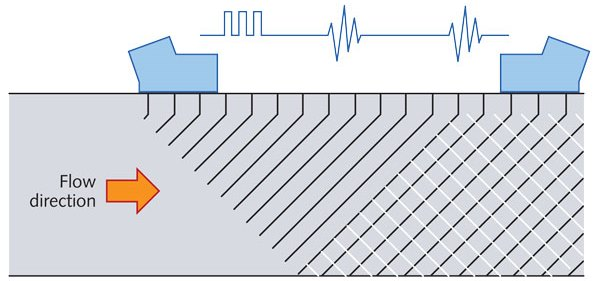
\includegraphics[scale=0.6]{figure/Lambsensors.jpg} 
\caption{ Schematic of actuator-sensor pair}
\end{figure}
\end{frame}
%%%%%%%%%%%%%%%%%%%%%%%%%%%%%%%%%
\begin{frame}{Lamb-wave propagation}
\begin{figure}
\includemovie[poster,text={\small(Loading Video...)}]{6cm}{4cm}{figure/video.avi}
\end{figure}
\end{frame}
%%%%%%%%%%%%%%%%%%%%%
\section{Problems associated with Lamb-wave}
\begin{frame}{Challenges}
\begin{itemize}
\item High dimensional.
\item Significant loss of information during feature.
 extraction process.
\item Use of multisensors can significantly improve the diagnosis process.
\end{itemize}
\end{frame}
%%%%%%%%%%%%%%%%%%%
\end{document}
